%===================================================================================================
%---------------------------------------------------------------------------------------------------
\subsection{Direct Shear Test}
%---------------------------------------------------------------------------------------------------
\Authors{TU Freiberg}
\todo{Please insert authors}

To conduct direct shear tests special equipment is necessary. The direct shear testing device at the rock mechanical laboratory of the TU Freiberg (see Fig. \ref{fig:ExpCNLShearMachine}) is specially developed to ensure the wanted functionality.\\

\begin{figure}[!ht]
\begin{center}
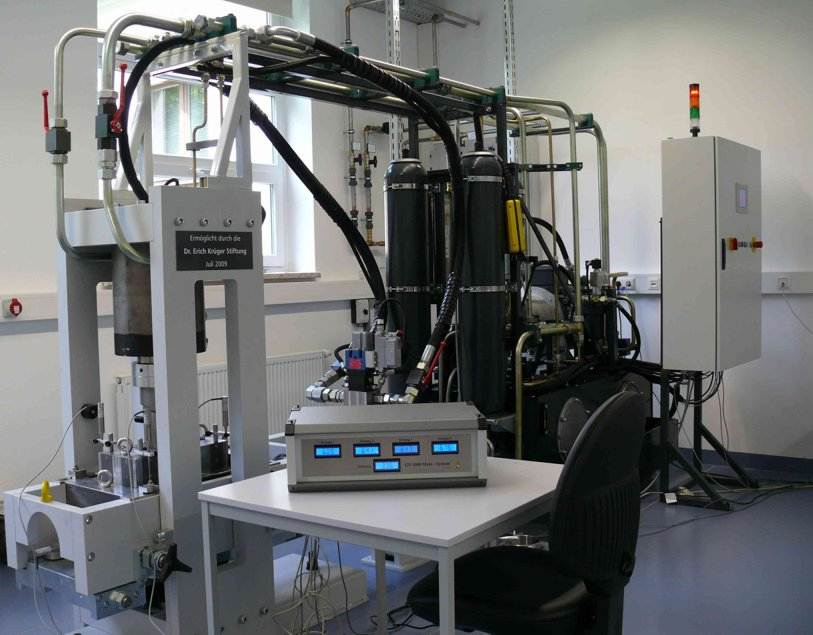
\includegraphics[width=0.5\textwidth]{./figures/ExpShearMachine.jpg}
\end{center}
\caption{The shear testing device at the rock mechanical laboratory at TU Freiberg. (From: \cite{Konietzky2012})}
\label{fig:ExpCNLShearMachine}
\end{figure}

Some key features can be found in Tab. \ref{table:ExpCNLDeviceTechnicalData}. Additionally it is possible to superimpose dynamic forces. In the tests for the GeomInt project this functionality wasn't used.\\

\begin{table}[!ht]
\begin{center}
\begin{tabular}{l r r}
feature & value & unit\\
\hline
Max. normal force & 1000 & kN\\
Max. shear displacement & 50 &mm\\
Min. shear velocity & 1e-7 & mm/s\\
Max. shear velocity & 70 & mm/s\\
Max. sample size (rectangular) & 200$\times$400 & mm\\
Max. fluid pressure & 10 & MPa\\
\end{tabular}
\caption{Technical data of the shear testing device. (From: \cite{Konietzky2012})}
\label{table:ExpCNLDeviceTechnicalData}
\end{center}
\end{table}

The sample preparation includes the cutting of the rock block in the cuboid shape. This sample is split into two parts and the rock joints are arranged in a matching position. It is arranged in the shear box, Fig. \ref{fig:ExpCNLSampleInShearBox}.\\


\begin{figure}[!ht]
\begin{center}
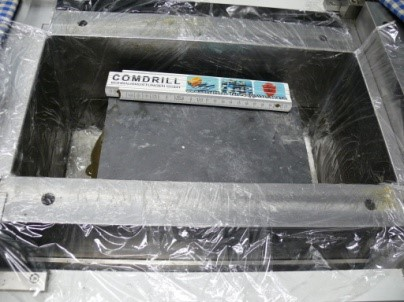
\includegraphics[width=0.5\textwidth]{./figures/ExpCNLSampleInShearBox.jpg}
\end{center}
\caption{Sample in shear box. (From: \cite{Nguyen2014})}
\label{fig:ExpCNLSampleInShearBox}
\end{figure}

The sample is grouted in the shear box to avoid any unwanted movements of it, Fig. \ref{fig:ExpCNLGroutedSample}.\\

\begin{figure}[!ht]
\begin{center}
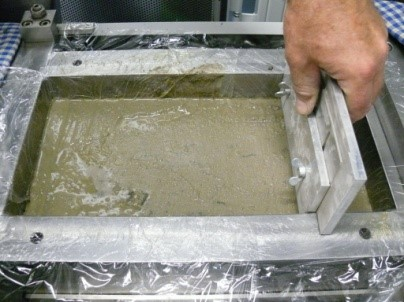
\includegraphics[width=0.5\textwidth]{./figures/ExpCNLGroutedSample.jpg}
\end{center}
\caption{Grouted sample before direct shear test. (From: \cite{Nguyen2014})}
\label{fig:ExpCNLGroutedSample}
\end{figure}

The finally equipped shear box is connected to the measuring units, the LVDTs (Linear Variable Differential Transformer), Fig. \ref{fig:ExpCNLLVDT}. The accuracy of this length measurements is in the order of $\unit[]{\mu m}$.

\begin{figure}[!ht]
\begin{center}
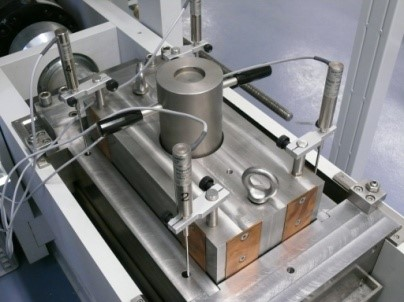
\includegraphics[width=0.5\textwidth]{./figures/ExpCNLLVDT.jpg}
\end{center}
\caption{Measuring equipment: LVDT. (From: \cite{Nguyen2014})}
\label{fig:ExpCNLLVDT}
\end{figure}

The set-up of the experiment is the same for CNL and CNS test. In the CNS test the stiffness which adds an extra load is calculated. This means if a normal displacement of the sample is measured the normal stress will be adapted according to the defined stiffness.


%\subsection{CNS Direct Shear Test (TU Freiberg)}
%---------------------------------------------------------------------------------------------------
\subsection{Cyclic Loading Pressure Diffusion}
\Authors{University of Stuttgart}
\todo{Please insert authors}

In order to study characteristic, time-dependent states of fractures under cycling loading conditions a sample is prepared with a single fracture and borehole before it is installed in a triaxial cell as shown in figure \ref{fig:exp_cyclic_pressure_triax}. The dimension of the sample are chosen to be $r = 30 \, \text{mm}$ and height $h = 70 \, \text{mm}$. 
\begin{figure}[!ht]
\begin{center}
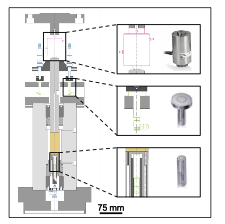
\includegraphics[width=0.5\textwidth]{./figures/exp_cyclic_pressure_triax.png}
\end{center}
\caption{Set-Up of triaxial cell.}
\label{fig:exp_cyclic_pressure_triax}
\end{figure}
The experiment is performed in three steps. After applying a confining pressure $p_{c}$ the initial state is approached by deformation control while the acting normal forces are measured in a first step. Once a desired normal force is reached the deformation state is held constant and a fluid pressure of $p_{fix}$ is applied. Finally, the fracture is stimulated by a harmonic fluid pressure with a frequency of $0.1 \, \text{Hz}$ and varying amplitudes $p_A$ between $0.5-3 \, \text{MPa}$. Throughout the experiment flow and pressure are measured at the fluid induction point to study the relationship of pressure and flow under non-constant fracture permeabilities triggered by deformations.